\begin{figure}[h!]
\centering
\begin{minipage}[c][5cm][t]{.5\textwidth}
\centering
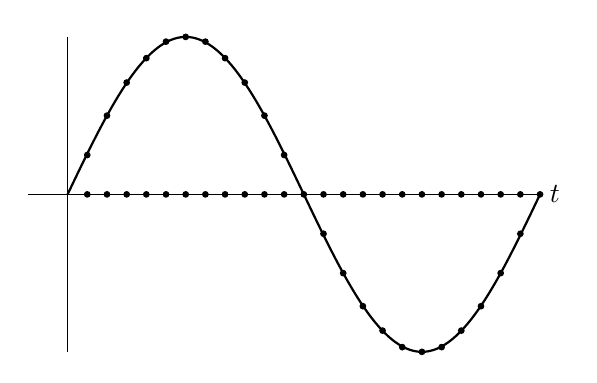
\begin{tikzpicture}
\shorthandoff{<>."}
  \draw[-] (-.5,0) -- (6,0) node[right] {$t$};
  \draw[-] (0,-2) -- (0,2) node[right] {$$};
  \draw [x=0.5cm,y=2cm, thick, black] (0,0) 
  sin (3,1) cos (6,0) sin (9,-1) cos (12,0);  
  \filldraw (0.25,0) circle (1pt);
  \filldraw (0.25,.5) circle (1pt);
  
  \filldraw (0.5,0) circle (1pt);
  \filldraw (0.5,1) circle (1pt);
  
  \filldraw (0.75,0) circle (1pt);
  \filldraw (0.75,1.42) circle (1pt);
  
  \filldraw (1,0) circle (1pt);
  \filldraw (1,1.73) circle (1pt);
    
  \filldraw (1.25,0) circle (1pt);
  \filldraw (1.25,1.94) circle (1pt);

  \filldraw (1.5,0) circle (1pt);
  \filldraw (1.5,2) circle (1pt);
  
  \filldraw (1.75,0) circle (1pt);
  \filldraw (1.75,1.94) circle (1pt);

  \filldraw (2,0) circle (1pt);
  \filldraw (2,1.73) circle (1pt);

  \filldraw (2.25,0) circle (1pt);
  \filldraw (2.25,1.42) circle (1pt);

  \filldraw (2.5,0) circle (1pt);
  \filldraw (2.5,1) circle (1pt);

  \filldraw (2.75,0) circle (1pt);
  \filldraw (2.75,.5) circle (1pt);

  \filldraw (3,0) circle (1pt);

  \filldraw (3.25,0) circle (1pt);
  \filldraw (3.25,-.5) circle (1pt);

  \filldraw (3.5,0) circle (1pt);
  \filldraw (3.5,-1) circle (1pt);

  \filldraw (3.75,0) circle (1pt);
  \filldraw (3.75,-1.42) circle (1pt);

  \filldraw (4,0) circle (1pt);
  \filldraw (4,-1.73) circle (1pt);

  \filldraw (4.25,0) circle (1pt);
  \filldraw (4.25,-1.94) circle (1pt);

  \filldraw (4.5,0) circle (1pt);
  \filldraw (4.5,-2) circle (1pt);

  \filldraw (4.75,0) circle (1pt);
  \filldraw (4.75,-1.94) circle (1pt);

  \filldraw (5,0) circle (1pt);
  \filldraw (5,-1.73) circle (1pt);

  \filldraw (5.25,0) circle (1pt);
  \filldraw (5.25,-1.42) circle (1pt);

  \filldraw (5.5,0) circle (1pt);
  \filldraw (5.5,-1) circle (1pt);

  \filldraw (5.75,0) circle (1pt);
  \filldraw (5.75,-.5) circle (1pt);

  \filldraw (6,0) circle (1pt);
  \shorthandon{<>."}
\end{tikzpicture}

\\a)
\end{minipage}%
\begin{minipage}[c][5cm][t]{.5\textwidth}
\centering
\begin{tikzpicture}
\shorthandoff{<>."}
  \draw[-] (-.5,0) -- (6,0) node[right] {$t$};
  \draw[-] (0,-2) -- (0,2) node[right] {$$};
  \draw (0.25,0) -- (0.25,.5);
  
  \draw (0.5,0) -- (0.5,1);
  
  \draw (0.75,0) -- (0.75,1.42);
  
  \draw (1,0) -- (1,1.73);
    
  \draw (1.25,0) -- (1.25,1.94);

  \draw (1.5,0) -- (1.5,2);
  
  \draw (1.75,0) -- (1.75,1.94);

  \draw (2,0) -- (2,1.73);

  \draw (2.25,0) -- (2.25,1.42);

  \draw (2.5,0) -- (2.5,1);

  \draw (2.75,0) -- (2.75,.5);

  \draw (3.25,0) -- (3.25,-.5);

  \filldraw (3.5,0) -- (3.5,-1);

  \filldraw (3.75,0) -- (3.75,-1.42);

  \filldraw (4,0) -- (4,-1.73);

  \filldraw (4.25,0) -- (4.25,-1.94);

  \filldraw (4.5,0) -- (4.5,-2);

  \filldraw (4.75,0) -- (4.75,-1.94);

  \filldraw (5,0) -- (5,-1.73);

  \filldraw (5.25,0) -- (5.25,-1.42);

  \filldraw (5.5,0) -- (5.5,-1);

  \filldraw (5.75,0) -- (5.75,-.5);

  \shorthandon{<>."}
\end{tikzpicture}

\\b)
\end{minipage}%
\caption[Proceso de muestreo]{En a) se toman muestras de una onda en intervalos de tiempo regulares $t$, en b) se hace una representaci\'on digital de la onda.}
\label{fig:muest}
\end{figure}